\chapter{Assoziationsdatenbank und Website}
Der Hauptteil von TIMA ist die Datenbank in denen die Assoziation gespeichert werden. Diese ist direkt verknüpft mir dem Webfrontend, dass sowohl der Hauptanlaufpunkt für die Benutzer ist als auch für die Apps durch die Bereitstellung einer umfassenden API.

Im nächsten Abschnitt wird das Backend und die Datenbank genauer beschrieben. Dabei wird genauer auf den Aufbau der einzelnen Tabellen eingegangen, sowie die verschiedenen Designentscheidungen.

Anschließend wird die API und die dahinter stehenden Designentscheidung genauer erläutert.

\section{Backend und Datenbank}
Für das Backend der Website haben für Django als grundlegende Technologie entschieden. Bei Django handelt es sich um ein in Python geschriebenes Webframework, das dem Model-View-Controller-Schema folgt. Django bietet unter anderem einen sehr komplexen objektrelationalen Mapper, der es ermöglicht auch komplexe Objektstrukturen abzubilden ohne die verwendete Datenbank explizit zu kennen.

\subsection{Datenmodell}
In \hyperref[fig:uml]{Abbildung \ref*{fig:uml}} ist das komplette Datenmodell von TIMA dargestellt. Dabei bildet das Modul \texttt{associations.models} den Kern.

\begin{figure}
	\centering
	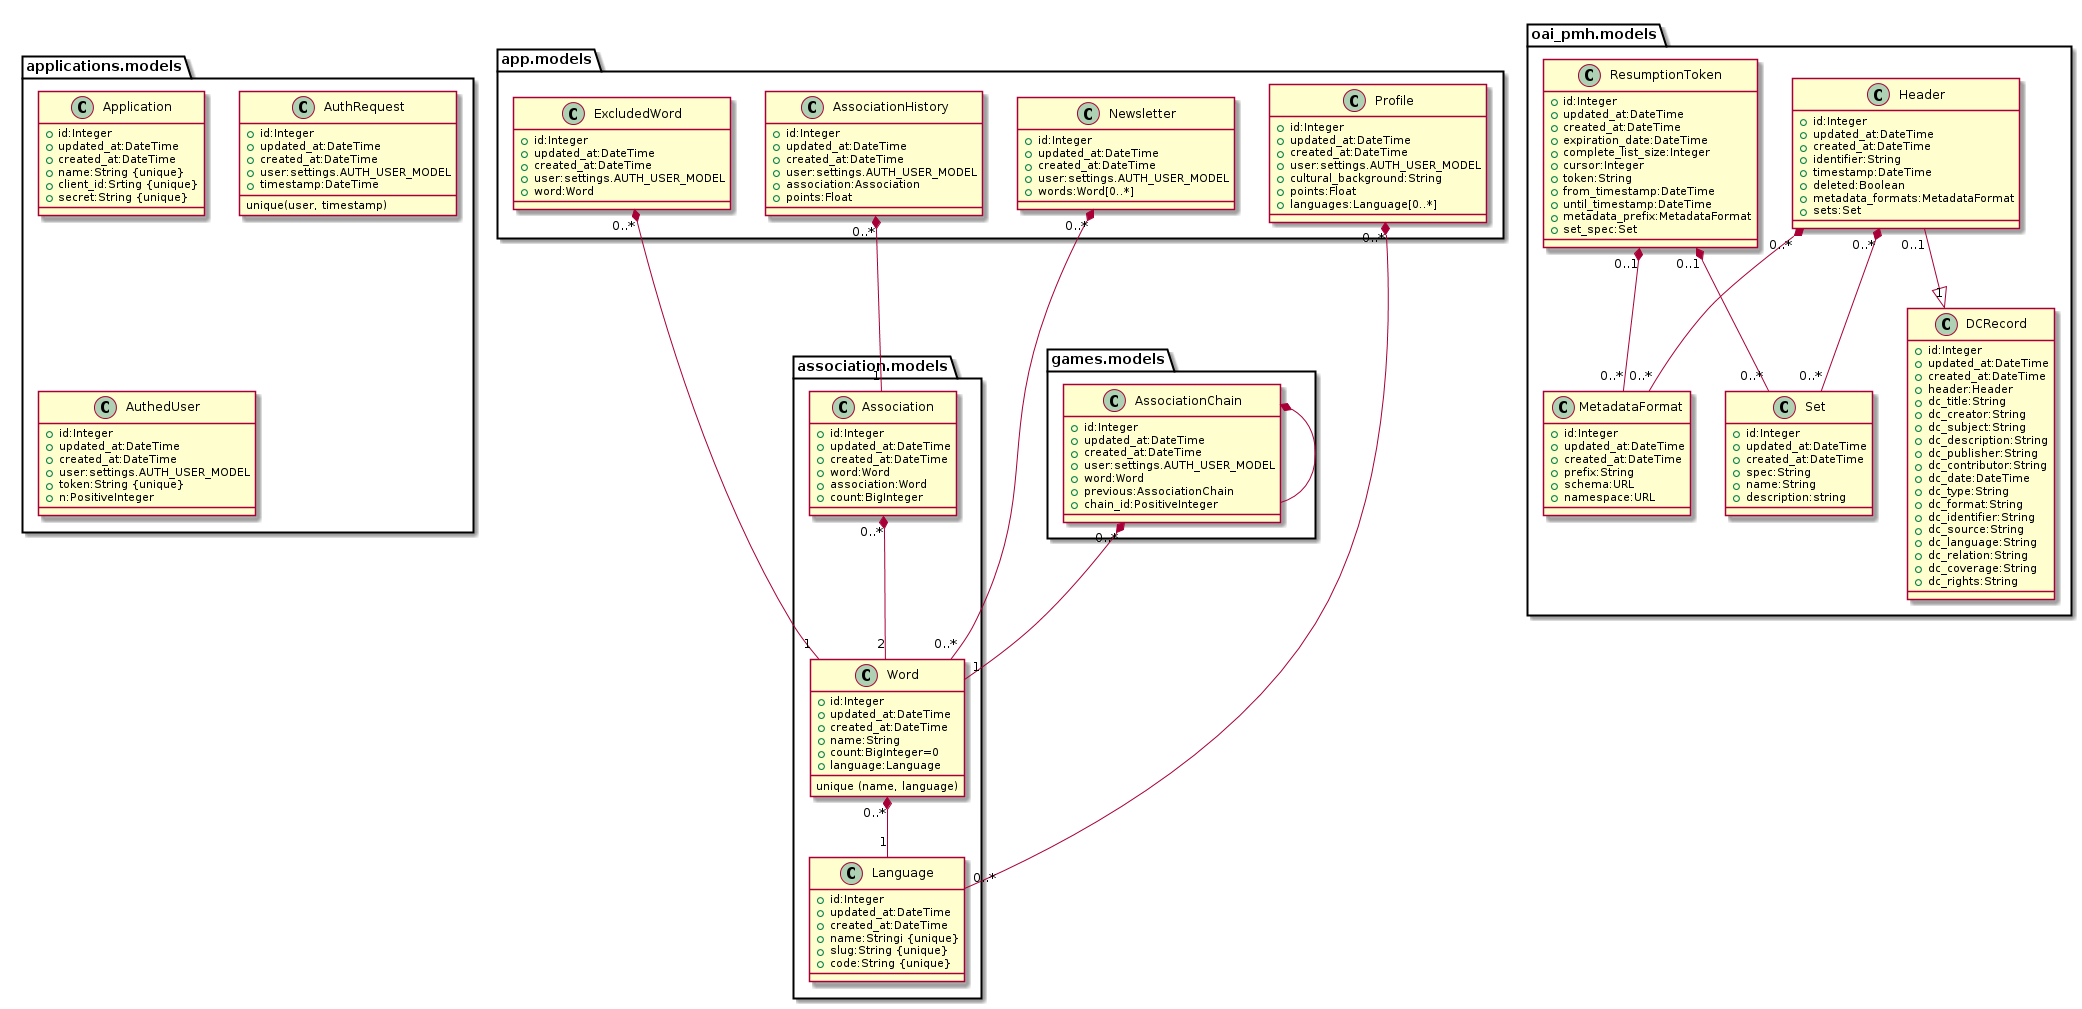
\includegraphics[width=\textwidth]{images/uml.png}
	\caption{UML des TIMA Datenmodells}
	\label{fig:uml}
\end{figure}

Das Modell \texttt{Language} repräsentiert die verfügbaren Sprachen der Wörter, das Modell \texttt{Word} die einzelnen Wörter, wobei ein Wort, wenn es in mehreren Sprachen existiert, für jede Sprache einen eigenen Eintrag hat und das Modell \texttt{Association} die Assoziation zwischen zwei Wörtern. Zusätzlich wird bei einem Wort gespeichert, wie oft dieses gefragt wurde und bei der Assoziation wir häufig diese gegeben wurde.

Die Modelle des Moduls \texttt{app.models} behandeln grundlegende Funktionen des Benutzermanagements. So zum Beispiel das Modell \texttt{Profile}, dass den Kulturellen Hintergrund, die Punktzahl und die Sprachen für die ein Benutzer assoziiert hat, speichert. In dem Modell \texttt{AssociationHistory} wird die gesamte Assoziationsgeschichte eines Benutzers gespeichert, mit den jeweils für eine Assoziation erhaltenen Punkte. Das Modell \texttt{ExcludeWord} enthält für jeden Benutzer die Wörter, die er übersprungen hat (siehe TODO ref), diese werden automatisch nach sieben Tagen gelöscht. Das letzte Modell in diesem Modul speichert für jeden Benutzer welche Worte er in seinem Newsletter empfangen möchte.

Das Modul \texttt{games.models} enthält Modelle die für verschiedenen Spiele wichtig sind. Dies ist im Moment nur AssoziationsKette (vgl. TODO ref), hierfür werden in dem Modul \texttt{AssociationChain} die letzte/aktuelle Assoziationskette eines Benutzer gespeichert. Diese wird bei jedem Start eines Spieles gelöscht.

Für die Kommunikation zwischen App und Backend, insbesondere die schreib Zugriffe (vgl. TODO ref), zu autorisieren und dem speichert der nötigen Informationen dient das Modul \texttt{applications.models}. Das Modell \texttt{Applicaion} speichert die Apps, die Autorisiert sind, mit den nötigen Daten für die Autorisierung (vgl TODO ref). Die beiden anderen Modell in diesem Modul \texttt{AuthRequest} und \texttt{AuthedUser} speichern die nötigen Information für einen Benutzer der sich authentifizieren möchte und hat.

Das letzte Modul und die beinhalteten Modell sind für das OAI-PMH erforderlich siehe dafür (TODO ref).

\section{Webfrontend}
Das Webfrontend ist die Hauptanlaufstelle für Benutzer. Hierüber kann sowohl anonym als auch angemeldet Assoziationen eingegeben, Wörter und deren Assoziationen angesehen und weitere Funktionen (Rangliste, Statistik) aufgerufen werden.

Das Webfrontend basiert auf Django, wurde zusätzlich zu HTML mit Bootstrap und JQuery erstellt, sowie zur Visualisierung D3.

\section{API}
API.md schöner schreiben, auth uml

bisschen OAI-PMH


